\title{ Angewandte Mathematik}
\author{Dr. Johannes Riesterer}
\date{\today}
\maketitle\thispagestyle{empty}
 \begin{figure}[H]
    \centering
    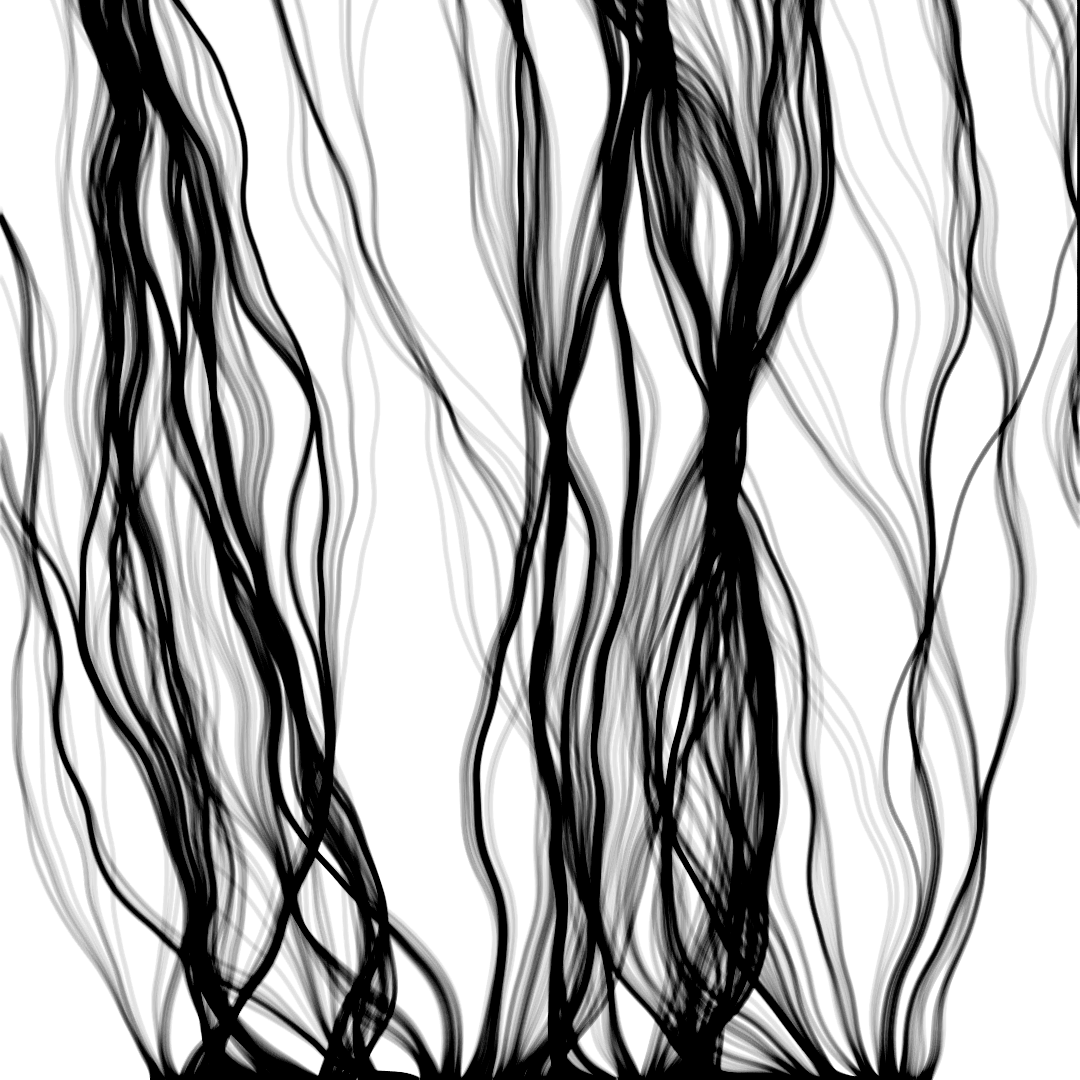
\includegraphics[width=1.0 \textwidth]{images/cover.png}
    \label{fig:diffus}
\end{figure}
\newpage 
\begin{center}
\large
 \copyright Johannes Riesterer \\
\end{center}
\thispagestyle{empty}
\newpage

\section*{Vorwort}
Kann jeder Mathematik lernen? Als Antwort auf diese Frage möchte ich auf den interessanten Lebenslauf
einer der bedeutendsten Mathematikerinnen aller Zeiten eingehen  (Auszug aus Wikipedia):

Emmy Noether war eine deutsche Mathematikerin, die grundlegende Beiträge zur abstrakten Algebra und zur theoretischen Physik lieferte. Insbesondere hat Noether die Theorie der Ringe, Körper und Algebren revolutioniert. Das nach ihr benannte Noether-Theorem gibt die Verbindung zwischen Symmetrien von physikalischen Naturgesetzen und Erhaltungsgrößen an. 

Sie zeigte in mathematischer Richtung keine besondere Frühreife, sondern hatte in ihrer Jugend Interesse an Musik und Tanzen. Sie besuchte die Städtische Höhere Töchterschule – das heutige Marie-Therese-Gymnasium – in der Schillerstraße in Erlangen. Mathematik wurde dort nicht intensiv gelehrt. Im April 1900 legte sie die Staatsprüfung zur Lehrerin der englischen und französischen Sprache an Mädchenschulen in Ansbach ab. 1903 holte sie in Nürnberg die externe Abiturprüfung am Königlichen Realgymnasium – dem heutigen Willstätter-Gymnasium – nach. 


\newpage
